\subsection{Idea}


Para la metaheurística de GRASP, tomaremos el algoritmo goloso previamente implementado y lo combinaremos con las diferentes búsquedas locales también previamente implementadas.

La idea es la siguiente, para cada paso del algoritmo, correremos una versión modificada del goloso de manera tal de permitir cierta aleatoriedad en los resultados. El algoritmo goloso será modificado de la siguiente manera:

\begin{algorithm}
  \begin{algorithmic}[1]\parskip=1mm
 \caption{ Goloso()}
 		\STATE{Numero los vértices de $1$ a $n$} 
		\STATE{Creo una cantidad $k$ de conjuntos donde iré guardando vértices}
 		\STATE{Para cada nodo $i$ de $1$ a $n$: }
		\STATE{\quad Para cada conjunto}
			\STATE{\quad\quad Sumo todos los pesos de las aristas de ($i$,$j$) con $j$ los vértices que están en el conjunto}
 		\STATE{\quad De los mejores $\alpha$ resultados, tomo uno al azar y pongo a $i$ en ese conjunto}
		\STATE{Devuelvo la respuesta}
\end{algorithmic}
\end{algorithm} 

Luego la RCL para cada nodo serán los $\alpha$ conjuntos para los cuales el peso es menor que agregarlo en cualquier otro conjunto. Notar que si $\alpha=1$ entonces estaríamos obteniendo el mismo algoritmo goloso que en el apartado anterior. En cambio, si tomo $\alpha = k$ (esto es, tomo los $k$ mejores resultados, o sea todos), estaría generando una solución completamente aleatoria. Cualquier solución en medio tomará una solución golosa, pero con cierto grado de aleatoriedad.

Otro posible criterio que consideramos fue buscar para cada nodo cual era el conjunto que minimizaba el peso de agregarlo en el mismo, y luego agregar en su RCL todos los conjuntos que estuvieran un porcentaje $\beta$ por sobre ese valor.

Finalmente y por cuestiones de tiempos se decidió solo implementar el primer algoritmo goloso descripto anteriormente.

Luego, a la solución obtenida por el algoritmo goloso randomizado, se le aplicarán una o varias de las búsquedas locales implementadas, en un intento de acercarnos aún más a la respuesta óptima.

Como criterio de corte se correrá el goloso aleatorizado y la busqueda local hasta que luego de que un número $z$, a determinar, de intentos no haya sido posible mejorar la solución. En este punto se entrega la mejor respuesta obtenida hasta el momento.

Teniendo a nuestra disposición tres búsquedas locales distintas, decidimos desarrollar tres GRASPs de tal manera que combinen de forma diferente estas búsquedas. El primero sólo utiliza la búsqueda local $1$, el segundo utiliza las tres búsquedas locales en orden descendente, es decir, primero la $3$, luego la $2$ y por último la $1$, y finalmente, el tercer y último GRASP utiliza dos búsquedas locales, en primer lugar la $3$ y luego la $1$. A continuación se formaliza de manera más precisa los algoritmos de cada uno:

\begin{algorithm}
  	\begin{algorithmic}[1]\parskip=1mm
		 \caption{ GRASP 1(SoluciónInicial) }
		 \STATE{while(true)}
		 	\STATE{\quad Corro el Algoritmo Goloso modificado}
		 	\STATE{\quad Utilizo búsqueda local 1 para mejorar la solución obtenida previamente}
		 	\STATE{\quad Si conseguí una mejor solución que antes, la guardo}
		 	\STATE{\quad Si tras $z$ iteraciones no se pudo conseguir una mejor solución}
		 	\STATE{\quad\quad Devuelvo la solución}
	\end{algorithmic}
\end{algorithm}

\begin{algorithm}
  	\begin{algorithmic}[1]\parskip=1mm
		 \caption{ GRASP 2(SoluciónInicial) }
		 \STATE{while(true)}
		 	\STATE{\quad Corro el Algoritmo Goloso modificado}
		 	\STATE{\quad Utilizo búsqueda local 3 para mejorar la solución obtenida previamente}
		 	\STATE{\quad Utilizo búsqueda local 2 para mejorar aún más la solución obtenida previamente}
		 	\STATE{\quad Utilizo búsqueda local 1 para nuevamente mejorar la solución obtenida previamente}
		 	\STATE{\quad Si conseguí una mejor solución que antes, la guardo}
		 	\STATE{\quad Si tras $z$ iteraciones no se pudo conseguir una mejor solución}
		 	\STATE{\quad\quad Devuelvo la solución}
	\end{algorithmic}
\end{algorithm}

\begin{algorithm}
  	\begin{algorithmic}[1]\parskip=1mm
		 \caption{ GRASP 3(SoluciónInicial) }
		 \STATE{while(true)}
		 	\STATE{\quad Corro el Algoritmo Goloso modificado}
		 	\STATE{\quad Utilizo búsqueda local 3 para mejorar la solución obtenida previamente}
		 	\STATE{\quad Utilizo búsqueda local 1 para mejorar aún más la solución obtenida previamente}
		 	\STATE{\quad Si conseguí una mejor solución que antes, la guardo}
		 	\STATE{\quad Si tras $z$ iteraciones no se pudo conseguir una mejor solución}
		 	\STATE{\quad\quad Devuelvo la solución}
	\end{algorithmic}
\end{algorithm}

En estos tres casos $z$ será un numero entero entre $1$ e infinito.

En el siguiente apartado de experimentación se intentarán calibrar tanto el parámetro $\alpha$ como el parámetro $z$ para así obtener los mejores resultados posibles con estas metaheurísticas, tratando siempre de equilibrar performance y exactitud de los resultados.

\subsection{Experimentación}

Para poder llegar a nuestro objetivo de encontrar los mejores parámetros $\alpha$ y $z$ a utilizar en las metaheurísticas, procederemos a hacer pruebas dejando fijo uno de los dos valores y variando el otro.
En primer lugar tomaremos un valor fijo arbitrario para $z$ y variaremos $\alpha$. Esta prueba consistirá en tomar un grafo y un $k$ fijo, y correr cada metaheurística con ese grafo como entrada y variando el parámetro $\alpha$. Una vez hecho esto, analizaremos para cuál valor de $\alpha$ se llegó a una mejor solución, es decir, el que más minimizó el peso total. Este parámetro $\alpha$ no podrá ser mayor que $k$ ya que si tengo $k$ conjuntos carece de sentido elegir entre los mejores $k'$ conjuntos siendo $k'>k$. Debido a lo previamente mencionado decidimos que $\alpha$ sea un porcentaje de $k$, que variaremos entre $0$ y $100$ saltando de a 10, es decir, $\alpha$ tomará los valores $0$, $10$, $20$,...,$90$ y $100$ 

Realizamos un primer experimento que consistió en lo siguiente:
Como primer paso generamos un grafo completo de $500$ nodos, con pesos en las aristas aleatorios enteros de $1$ a $100$, con $k=100$. Luego para cada valor de $\alpha$ corrimos los tres GRASPs. Para cada uno de los GRASPs se obtuvo un $\alpha$ ganador, es decir, el $\alpha$ que minimizó el peso en cada caso. Este proceso se realizó $100$ veces, siempre generando un grafo completo con pesos distintos en las aristas y en cada caso consiguiendo un $\alpha$ ganador. A continuación se presenta un gráfico, en cual se encuentran los tres GRASPs, que muestra para cada $\alpha$ cuántas de las 100 veces "ganó". 

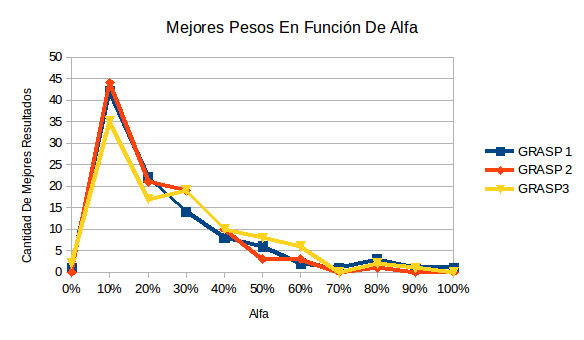
\includegraphics[scale=0.7]{Ej5/respuestasAlfa1.png}\\

Por lo que se ve en el gráfico, puede inferirse que para $\alpha=10$ se logran los mejores resultados en los tres GRASPs, al menos para el caso de 500 nodos. Para no quedarnos solamente con esta prueba, realizamos este mismo experimento nuevamente pero esta vez con $1000$ nodos y $k=200$. A continuación el gráfico correspondiente.

%ACÁ EL GRÁFICO DE LOS 3 GRASP PARA 1000 NODOS

Los resultados son claros, nuevamente $\alpha=10$ es el ganador. Con esto podemos concluir con cierto grado de seguridad que el mejor valor para $\alpha$ es $10$.

%------------------REVISAR ESTO---------------------
Respecto al tiempo que tardan los algoritmos, para los 100 grafos antes mencionados, tambien medimos el tiempo que tardaron, aquí se puede ver en promedio cuanto tardó cada uno:

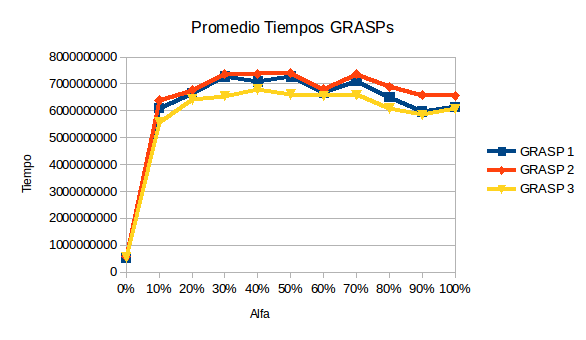
\includegraphics[scale=0.7]{Ej5/tiemposAlfa.png}\\

No se aprecian diferencias significativas, salvo con $\alpha$ igual a 0, ya que este a decir verdad no es un GRASP ya que no tiene aleatoriedad al momento de elegir a donde irá el nodo.

%En realidad me parece que con un menor numero de cuantosMejores debería tardar menos... pero hay que fijarse lo que dieron las pruebas.

Observando las soluciones que se obtienen eligiendo el mejor valor para $\alpha$ y no otro valor, se obtienen mejoras que varían entre $1\%$ y $9\%$. Para ejemplificar, lo que queremos decir se muestra en el siguiente grafico, los distintas soluciones soluciónes que arrojó el GRASP 1 sobre un mismo grafo y variando el $\alpha$:

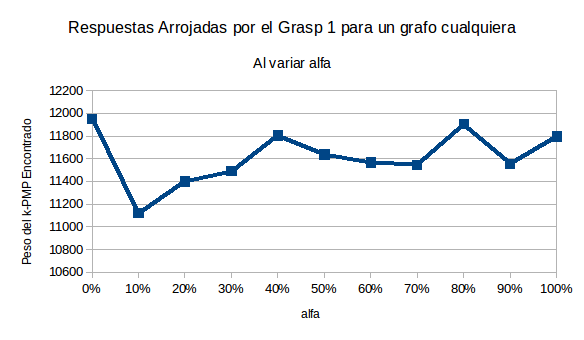
\includegraphics[scale=0.7]{Ej5/ejemploAlfa.png}\\

%------------------REVISAR ESTO---------------------

Una vez obtenido el mejor valor para $\alpha$, pasamos a buscar el mejor valor para $z$, con lo cual dejaremos fijo $\alpha=10$ y variaremos el $z$.

Realizamos el segundo experimento, el cual consistió en tomar grafos completos de $250$ nodos y $k = 70$ variando $z$ desde $z = 4$ hasta $z = 40$ (para valores mayores de $z$ los tiempos de ejecución resultaban excesivos) para ver como respondía la metaheuristica ante estos cambios. Luego a los valores obtenidos de k-MPM se promedian para ver como varían en promedio los resultados al variar este parametro.
Los resultados pueden verse aquí:

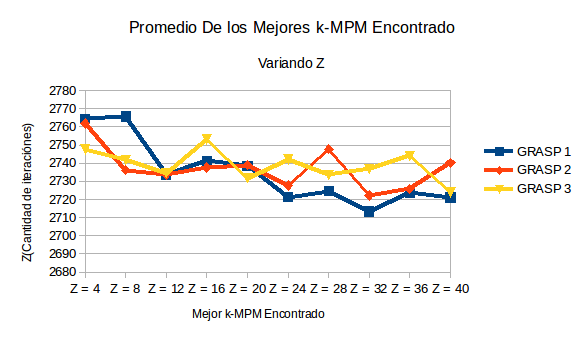
\includegraphics[scale=0.7]{Ej5/promedioZ.png}\\

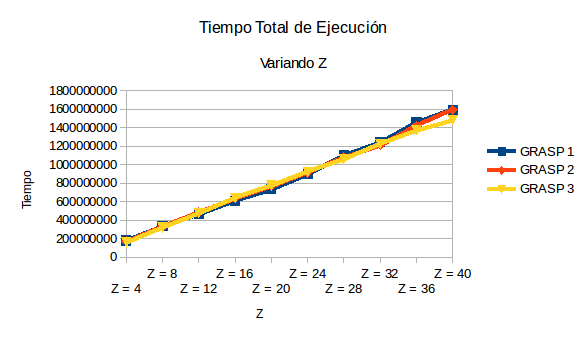
\includegraphics[scale=0.7]{Ej5/tiemposZ.png}\\

Como se puede ver en el grafico de tiempos, al aumentar la cantidad de iteraciones aumenta de manera lineal el tiempo de ejecución. Sin embargo las respuestas arrojadas por los algoritmos no mejoran con la misma pendiente, sinó que lo hacen con una mucho mas moderada. Se decide tomar $z = 34$ para los tres GRASPs que se considera un valor que equilibra tanto las respuestas obtenidas, como un tiempo de ejecución apropiado. 

Finalmente con estos valores para $\alpha$ y $z$, realizamos un último experimento para comparar las soluciones y los tiempos de cada GRASP.

Este último experimento consistió en, tomando $100$ nuevos grafos completos de $150$ nodos y con $k = 7$ y pesos aleatorios en sus aristas que varíen entre $1$ y $100$. Ver cual de los tres algoritmos es el que obtiene mejores resultados.

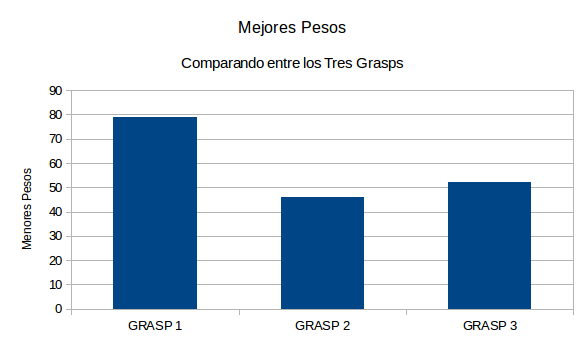
\includegraphics[scale=0.7]{Ej5/CompetenciaGRASPs1.png}\\

Dicho con palabras, entre los GRASPs, el GRASP 1 encontró 79 veces la menor solución (comparandolo con GRASP 2 y GRASP 3), el GRASP 2 la encontró 46 veces y el GRASP 3, 52. El hecho de que la suma de mayor a $100$ proviene de que en varias ocaciones mas de un algoritmos encontró la menor solución.

Idem para $250$ nodos, $k = 40$

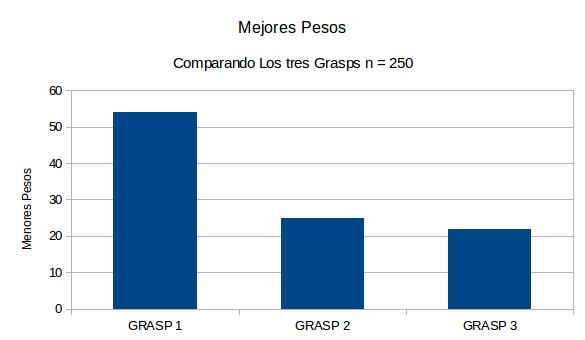
\includegraphics[scale=0.7]{Ej5/CompetenciaGRASPs2.png}\\

Idem para $500$ nodos, $k = 70$

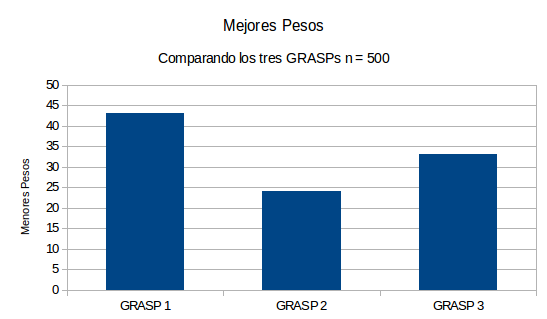
\includegraphics[scale=0.7]{Ej5/CompetenciaGRASPs3.png}\\

Luego, tras todo este testeo podemos concluír que el GRASP $1$ es mejor para un numero mayor de casos que los otros dos algoritmos implementados.

En la sección siguiente utilizaremos el GRASP 1 y lo compararemos contra los otros algoritmos implementados. Asi podremos obtener resultados mas precisos de cuanto por encima de la solución exacta se encuentra, sobre que tipo de grafos es conveniente usarlo, etc.